\documentclass[a4j, titlepage]{jsarticle}
\usepackage[dvipdfmx]{graphicx}
\usepackage{amsmath,ascmac,amsthm, amssymb}
\usepackage{amsfonts,latexsym,mathtools}
\usepackage{bm}
\usepackage{algorithm,algorithmic}
\usepackage{listings}
\usepackage{empheq}
\lstset{
    language={C},
    basicstyle={\small\ttfamily},
    identifierstyle={\small},
    commentstyle={\small\itshape},
    keywordstyle={\small\bfseries},
    ndkeywordstyle={\small},
    stringstyle={\small\ttfamily},
    frame={tb},
    breaklines=true,
    columns=[l]{fullflexible},
    numbers=left,
    xrightmargin=0zw,
    xleftmargin=3zw,
    numberstyle={\scriptsize},
    stepnumber=1,
    numbersep=1zw,
    lineskip=-0.5ex
}
\renewcommand{\lstlistingname}{コード}
\renewcommand{\lstlistlistingname}{コード目次}

\numberwithin{equation}{section}
%\setcounter{tocdepth}{3}

\begin{document}
\begin{titlepage}
    \begin{center}
        {\Large 令和四年度後期 数理工学実験 課題レポート}

        \vspace*{180truept}

        {\Huge 連続最適化}

        \vspace{160truept}

        {\Large 情報学科2回生 平田蓮}

        \vspace{10truept}

        {\large 学生番号: 1029342830}

        \vspace{60truept}

        {\large 実験日: 11月29, 12月5, 6, 12日}

        \vspace{10truept}

        {\large 実験場所: 京都大学工学部総合校舎数理計算機室}

        \vspace{60truept}

        {\large 12月19日 提出}
    \end{center}
\end{titlepage}

\tableofcontents
\clearpage

\section{目的}
    本実験では連続な関数についての最適化手法を学び、それに関する演習をPythonを用いて行う。
    \ref{sec:kadai1}節では関数の零点探索、
    \ref{sec:kadai2}では1変数関数の停留点探索を行い、
    \ref{sec:kadai3}, \ref{sec:kadai4}, \ref{sec:kadai5}節では
    2変数関数における最適化問題解く。

\section{課題}
    \subsection{課題1} \label{sec:kadai1}
        まず、本課題で用いるアルゴリズム、二分法とニュートン法について説明する。
        これらはどちらも連続な1変数関数$f: \mathbb{R} \rightarrow \mathbb{R}$における零点
        ($x \in \mathbb{R} \ \mathrm{s.t.} \ f(x)=0$)
        を探索するアルゴリズムである。

        \subsubsection{二分法}
            初期値として、$f(a) < 0, f(b) \geq 0$を満たす$a, b \in \mathbb{R}$を選ぶ。
            $f$は連続なので、零点が$a$と$b$の間に存在する。
            よって、これらの中点$\displaystyle x=\frac{a+b}{2}$と$a, b$を
            置き換えながら範囲を狭めていくことで零点を探索する。
            このアルゴリズムは次のように書ける。
            \begin{enumerate}
                \item 探索範囲の境界$a, b$について、中点$x=\displaystyle\frac{a+b}{2}$を計算
                \item $f(x)<0$なら$a \leftarrow x$、そうでないなら$b\leftarrow x$
                \item $|a-b|$が一定の値を下回るまで繰り返す
            \end{enumerate}

        \subsubsection{ニュートン法}
            適当な初期値$x_k$を取る。
            $f(x)$を$x_k$の周りで一次関数で近似し、
            それと$x$軸の交点を新しい$x_k$とする。
            このアルゴリズムは次のように書ける。
            \begin{enumerate}
                \item $x_k$について、$y=f'(x_k)(x-x_k)+f(x_k)$を考える
                \item $y=0$となる$x=x_k-\displaystyle\frac{f(x_k)}{f'(x_k)}$について、$x_k\leftarrow x$
                \item $|f(x_k)|$が一定の値を下回るまで繰り返す
            \end{enumerate}

        以下では$f=x^3+2x^2-5x-6$について考える。

        \subsubsection{課題 (a)}
            $f$を$-10\leq x,y\leq 10$の範囲で描画する。
            作成したソースコードをリスト\ref{src:1f}, \ref{src:1fview}に示す。
            \begin{lstlisting}[caption=$f$の実装, label=src:1f]
class Function:
    def __call__(self, x:float) -> float:
        return x**3 + 2 * x**2 - 5 * x - 6

    def __str__(self) -> str:
        return '$f = x^3 + 2x^2 - 5x - 6$'

    def df(self, x:float): # 微分
        return 3 * x**2 + 4 * x - 5
            \end{lstlisting}
            \begin{lstlisting}[caption=$f$を描画するソースコード, label=src:1fview]
import numpy
from matplotlib import pyplot


pyplot.rcParams["text.usetex"] = True
pyplot.rcParams["font.size"] = 12


def plot(
    f:Function,
    xlim:tuple[int],
    ylim:tuple[int],
    save_path:str,
    n=10**7
) -> None:
    x = numpy.linspace(*xlim, n)
    pyplot.plot(x, f(x), label=str(f))
    
    pyplot.xlim(xlim)
    pyplot.ylim(ylim)

    pyplot.xlabel('$x$')
    pyplot.ylabel('$f$', rotation=0)
    
    pyplot.grid()
    pyplot.legend()
    pyplot.savefig(save_path)


if __name__ == '__main__':
    f = Function()
    plot(f, xlim=(-10, 10), ylim=(-10, 10), save_path='a.pdf')                
            \end{lstlisting}

            描画した結果を図\ref{fig:1fview}に示す。

            \begin{figure}[h]
                \centering
                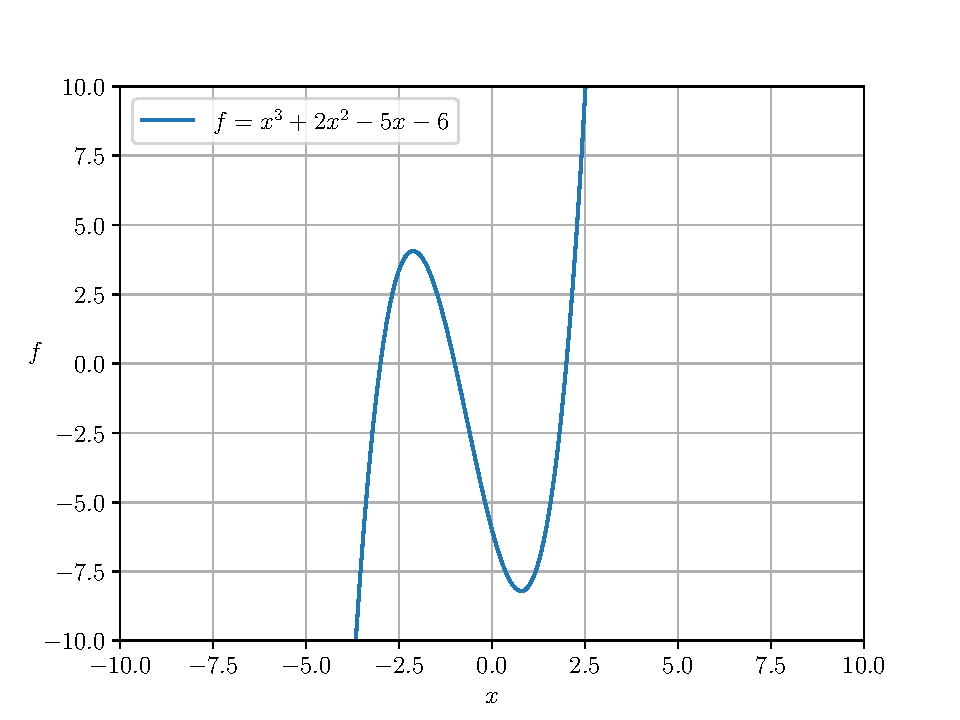
\includegraphics[width=0.8\hsize]{kadai1/a.pdf}
                \caption{$f$の描画結果}
                \label{fig:1fview}
            \end{figure}

        \subsubsection{課題 (b)}
            二分法を用いて$f$の零点を全て求める。
            図\ref{fig:1fview}より、$f$の零点は
            -5と-2.5の間、-2.5と0の間、0と2.5の間にそれぞれあることがわかるので、
            これらを初期値に用いる。
            作成したソースコードをリスト\ref{src:1bin}に示す。
            今回は、$|a-b|\leq 10^{-7}$になるまで反復する。

            \begin{lstlisting}[caption=二分法の実装, label=src:1bin]
def get_zero_points(
    algorithm:Callable,
    f:Function,
    starts:list
) -> list[float]:
    return [algorithm(f, start) for start in starts]

def get_zero_point_with_bisection(
    f:Function, start:tuple[float],
    terminate_threshold:float=10**-7
) -> list[float]:
    left:float
    right:float
    left, right = start
    
    assert f(left) * f(right) <= 0
    
    mid:float = None
    mids:list[float] = []
    while abs(left - right) > terminate_threshold:
        mid = (left + right) / 2
        mids.append(mid)
        if f(mid) * f(left) > 0:
            left = mid
        else:
            right = mid
            
    mids.append(mid)
    return mids


if __name__ == '__main__':
    f:Function = Function()
    zero_points:list[float] = get_zero_points(get_zero_point_with_bisection, f, starts=[
        (-5, -2.5),
        (-2.5, 0),
        (0, 2.5)
    ])
            \end{lstlisting}

            \verb|get_zero_point_with_bisection()|は、
            最終的な零点だけでなく、反復時の$\displaystyle\frac{a+b}{2}$の遷移を返す。

            求めた零点を図\ref{fig:1fzero}に示す。
            \begin{figure}[h]
                \centering
                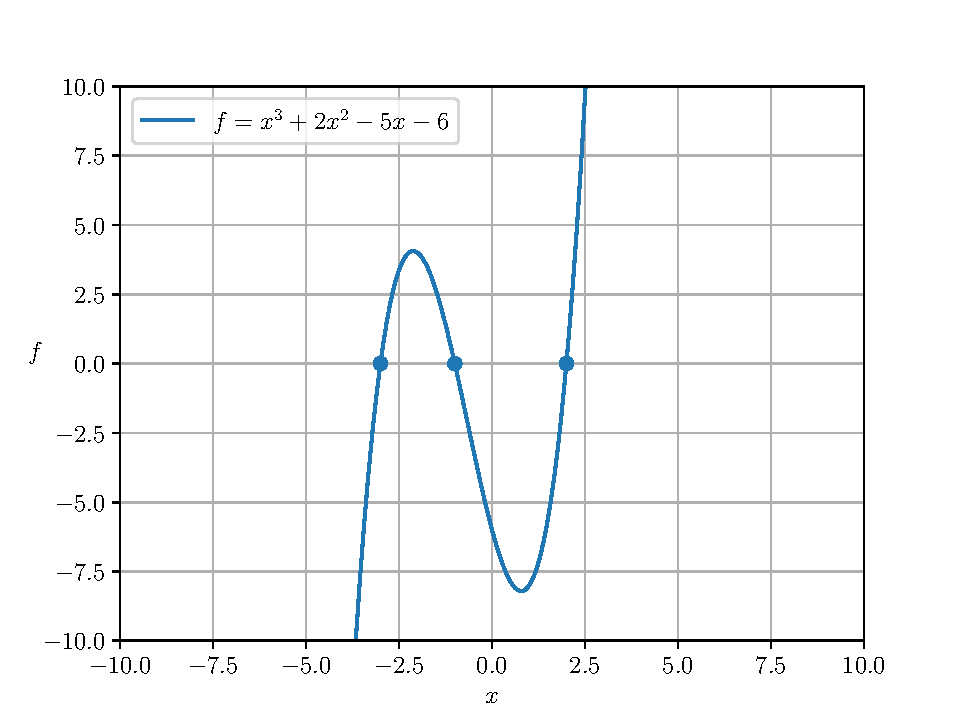
\includegraphics[width=0.8\hsize]{kadai1/b.pdf}
                \caption{$f$の零点}
                \label{fig:1fzero}
            \end{figure}

            零点は$x=-3,-1,2$であった。
            図より実際にこれらが零点となっていることがわかる。

        \subsubsection{課題 (c)}
            ニュートン法を用いて$f$の零点を用いる。
            ニュートン法の初期値は、零点の十分近くを取らないと収束しないことが知られているため、
            今回は$x=-4,0,4$を用い、
            $|f(x)|\leq 10^{-7}$になるまで反復した。
            作成したソースコードをリスト\ref{src:1newton}に示す。

            \begin{lstlisting}[caption=ニュートン法の実装, label=src:1newton]
def get_zero_point_with_newton(
    f:Function,
    start:float,
    terminate_threshold:float=10**-7
) -> list[float]:
    x:float = start
    xs:list[float] = []
    while abs(f(x)) > terminate_threshold:
        xs.append(x)
        x -= f(x) / f.df(x)
        
    xs.append(x)
    return xs


if __name__ == '__main__':
    f:Function = Function()
    zero_points:list[float] = get_zero_points(get_zero_point_with_newton, f, starts=[
        -4,
        0,
        4
    ])
            \end{lstlisting}

            二分法と同様の結果が得られたため、結果は省略する。

        \subsubsection{考察}
            零点の理論解$x_0$と、探索による値$x$の誤差を
            $E=|x_0-x|$と定義する。
            各種法における反復回数$k$回時点の$x$について、$E$をプロットした図を
            図\ref{fig:1fe0}, \ref{fig:1fe1}, \ref{fig:1fe2}に示す。

            \begin{figure}[h]
                \centering
                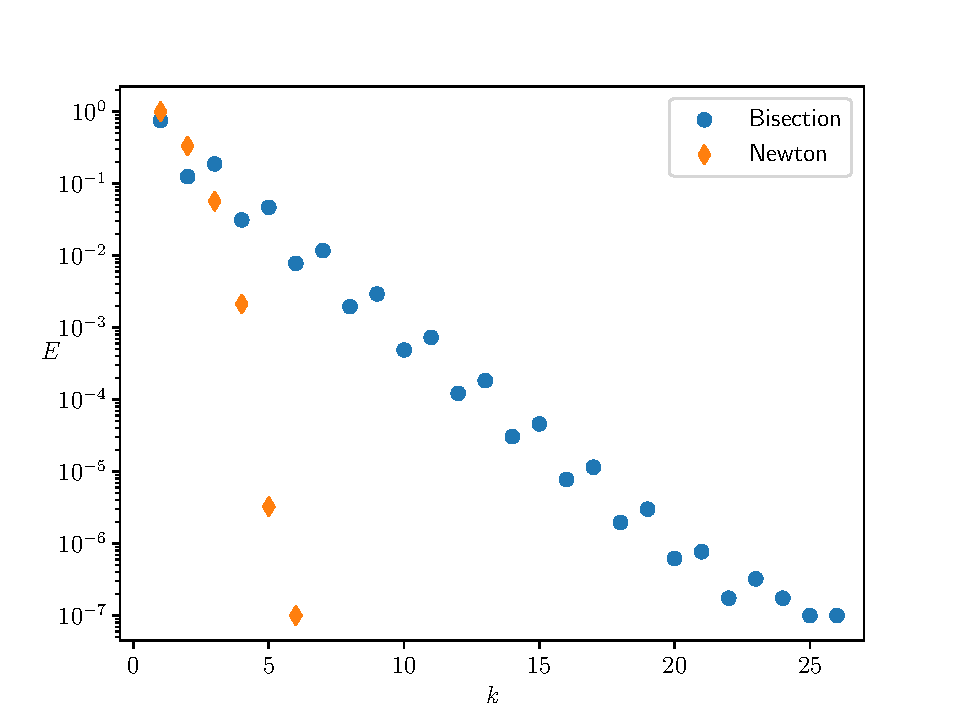
\includegraphics[width=0.8\hsize]{kadai1/change0.pdf}
                \caption{
                    零点$x=-3$と探索解の誤差。
                    Bisectionが二分法、Newtonがニュートン法を示す。
                }
                \label{fig:1fe0}
            \end{figure}
            \begin{figure}[h]
                \centering
                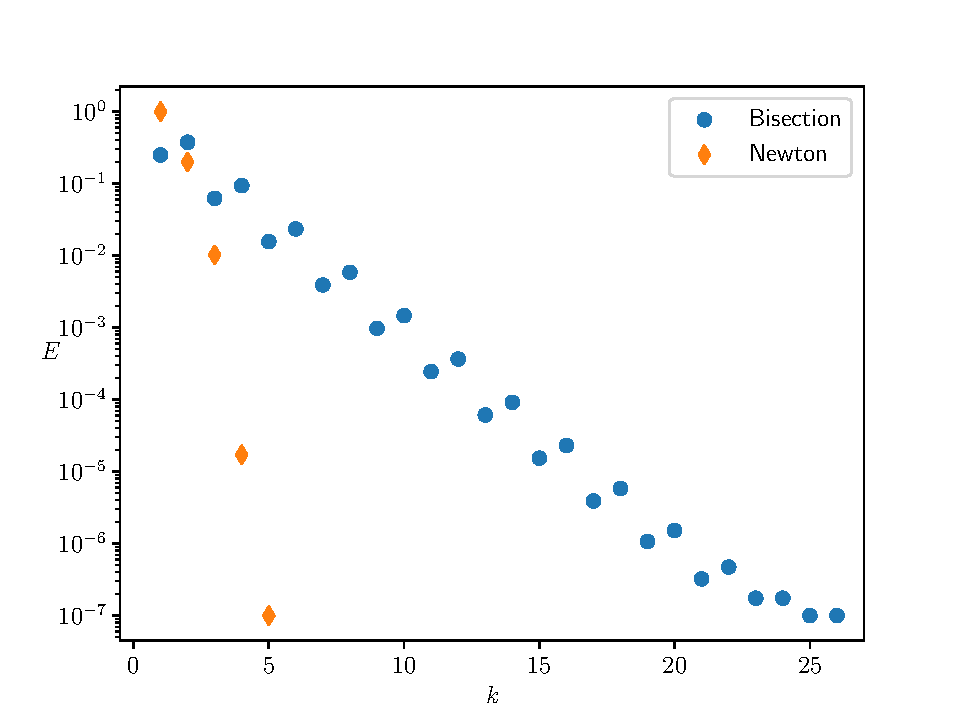
\includegraphics[width=0.8\hsize]{kadai1/change1.pdf}
                \caption{
                    零点$x=-1$と探索解の誤差。
                    Bisectionが二分法、Newtonがニュートン法を示す。
                }
                \label{fig:1fe1}
            \end{figure}
            \begin{figure}[h]
                \centering
                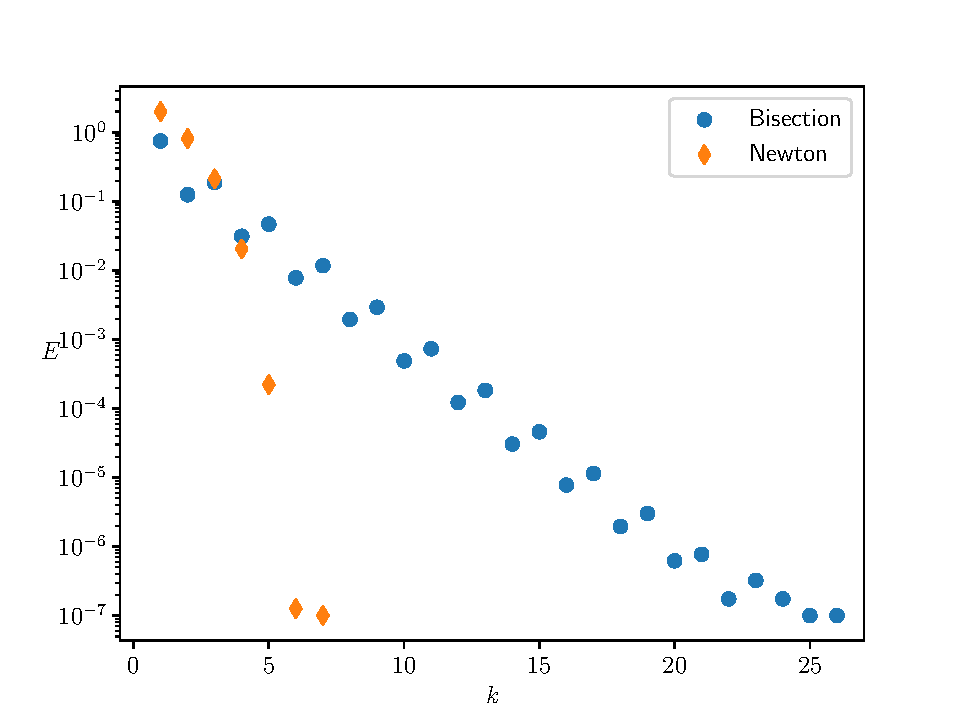
\includegraphics[width=0.8\hsize]{kadai1/change2.pdf}
                \caption{
                    零点$x=2$と探索解の誤差。
                    Bisectionが二分法、Newtonがニュートン法を示す。
                }
                \label{fig:1fe2}
            \end{figure}

            三つの図より、ニュートン法の方が二分法と比べて早く結果が収束していることがわかる。

    \subsection{課題2} \label{sec:kadai2}
        はじめに、本課題で用いるアルゴリズム、最急降下法と
        ニュートン法の拡張について説明する。

        \subsubsection{最急降下法}
            ニュートン法のように、$x\leftarrow x+td_k$
            と$x$を更新しながら値を探索するアルゴリズムを降下法と呼ぶ。
            ここで、$t$はステップ幅、$d_k$は変化方向である。
            最急降下法は次に示す最急降下方向を用いることで関数の停留点を求めることができる。
            \begin{equation*}
                最急降下方向 d_k=-\nabla f(x)
            \end{equation*}

        \subsubsection{ニュートン法の拡張}
            次に示すニュートン方向を用いた降下法でも、関数の停留点を求めることができる。
            \begin{equation*}
                ニュートン方向 d_k=-\nabla^2f(x)^{-1}\nabla f(x)
            \end{equation*}
            ここで、$\nabla^2f(x)$は$f$のヘッセ行列である。

        以下では関数$f=\displaystyle\frac{x^3}{3}-x^2-3x+\frac{5}{3}$を考える。

        \subsubsection{課題 (a)} \label{sec:2a}
            最急降下法を用いて$f$の停留点を求める。
            初期値は$x=0.5$, $k$ステップ目$(k=0,1,\cdots)$においてステップ幅は
            $\displaystyle t=\frac{1}{k+1}$とする。
            反復の終了条件は$|\nabla f(x)| \leq 10^{-7}$とした。

            作成したソースコードをリスト\ref{src:2f}, \ref{src:2saikyu}に示す。

            \begin{lstlisting}[caption=$f$の実装, label=src:2f]
class Function:
    def __call__(self, x:float) -> float:
        return x**3 / 3 - x**2 - 3 * x + 5 / 3
    
    def __str__(self) -> str:
        return r'$\displaystyle\frac{1}{3}x^3 - x^2 - 3x + \frac{5}{3}$'
    
    def df(self, x:float): # 一階微分
        return x**2 - 2 * x - 3
    
    def d2f(self, x:float): # 二階微分
        return 2 * x - 2
            \end{lstlisting}

            \begin{lstlisting}[caption=最急降下法の実装, label=src:2saikyu]
def get_critical_point_with_gradient(
    f:Function,
    start:float,
    terminate_threshold:float=10**-7
) -> list[float]:
    x:float = start
    k = 0
    
    xs:list[float] = [x]
    last_f:float = float('inf')
    while abs(last_f - f(x)) > terminate_threshold:
        last_f = f(x)
        x -= f.df(x) * 1 / (k + 1)
        
        xs.append(x)
        k += 1
    
    return xs


if __name__ == '__main__':
    f:Function = Function()
    critical_point:list[float] = get_critical_point_with_gradient(f, 1/2)
            \end{lstlisting}

            求めた停留点を図\ref{fig:2f}に示す。

            \begin{figure}[h]
                \centering
                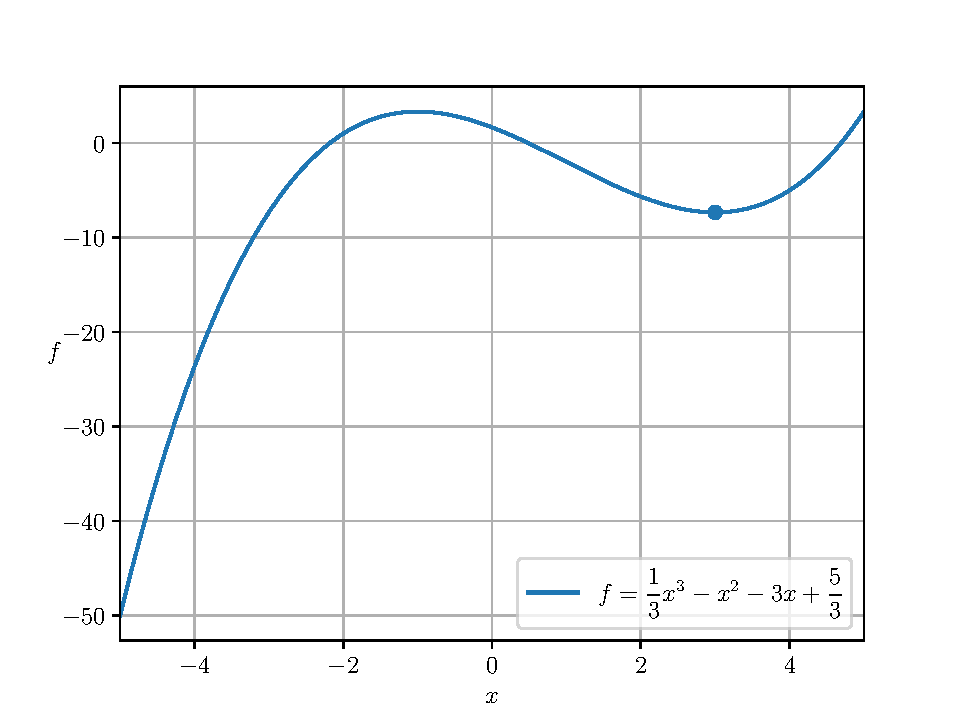
\includegraphics[width=0.8\hsize]{kadai2/a.pdf}
                \caption{$f$の停留点}
                \label{fig:2f}
            \end{figure}

            停留点は$x=3$と求まり、これが正しいことが図よりわかる。

        \subsubsection{課題 (b)} \label{sec:2b}
            ニュートン法を用いて$f$の停留点を求める。
            初期値は$x=5$,
            ステップ幅は$t=k$とする。
            終了条件は$|\nabla^2f(x)^{-1}\nabla f(x)|\leq 10^{-7}$とした。

            作成したソースコードをリスト\ref{src:2fnewton}に示す。

            \begin{lstlisting}[caption=ニュートン法の実装, label=src:2fnewton]
def get_critical_point_with_newton(
    f:Function,
    start:float,
    terminate_threshold:float=10**-7
) -> list[float]:
    x:float = start
    k = 0
    
    xs:list[float] = [x]
    last_f:float = float('inf')
    while abs(last_f - f(x)) > terminate_threshold:
        last_f = f(x)
        x -= f.df(x) / f.d2f(x)
        
        xs.append(x)
        k += 1
    
    return xs


if __name__ == '__main__':
    f:Function = Function()
    critical_point:list[float] = get_critical_point_with_newton(f, 5)
            \end{lstlisting}

            最急降下法と同様の結果が得られたため、結果は省略する。

    \subsection{課題3} \label{sec:kadai3}
        次の最適化問題を考える。
        \begin{eqnarray*}
            \mathrm{minimize} \ f(\bm{x}) &=& x_0^2 + e^{x_0} + x_1^4 + x_1^2 -2x_0x_1 + 3 \\
            \bm{x} &=& \begin{pmatrix}
                x_0 \\
                x_1
            \end{pmatrix} \in \mathbb{R}^2
        \end{eqnarray*}

        $\nabla f(x), \nabla^2f(x)$は、
        次の形で表せる。
        \begin{eqnarray*}
            \nabla f(x) &=& \begin{pmatrix}
                2x_0 + e^{x_0} - 2x_1 \\
                4x_1^3 + 2x_1 - 2x_0
            \end{pmatrix} \\
            \nabla^2f(x) &=& \begin{pmatrix}
                2 + e^{x_0} & -2 \\
                -2 & 12x_1^2+2
            \end{pmatrix}
        \end{eqnarray*}

        $f(x), 勾配\nabla f(x), ヘッセ行列\nabla^2f(x)$を出力するソースコードを
        リスト\ref{src:3f}に示す。

        \begin{lstlisting}[caption={$f, \nabla f, \nabla^2f$の実装}, label=src:3f]
import numpy

class Function:
    def __call__(self, x:tuple[float]) -> float: # f
        assert 2 == len(x)
        return x[0]**2 + numpy.exp(x[0]) + x[1]**4 + x[1]**2 - 2 * x[0] * x[1] + 3
    
    def __str__(self) -> str:
        return r'$\displaystyle\frac{1}{3}x^3 - x^2 - 3x + \frac{5}{3}$'
    
    def df(self, x:tuple[float]) -> numpy.array: # 勾配ベクトル
        assert 2 == len(x)
        return numpy.array([
            2 * x[0] + numpy.exp(x[0]) - 2 * x[1],
            4 * x[1]**3 + 2 * x[1] - 2 * x[0]
        ])
    
    def d2f(self, x:tuple[float]) -> numpy.matrix: # ヘッセ行列
        assert 2 == len(x)
        return numpy.matrix([
            [2 + numpy.exp(x[0]), -2],
            [-2, 12 * x[1]**2 + 2]
        ])
        \end{lstlisting}

    \subsection{課題4} \label{sec:kadai4}
        反復時のステップ幅$t_k$を適切に計算するアルゴリズム、
        バックトラック法を説明する。

        \subsubsection{バックトラック法}
            バックトラック法はステップ幅$t$を用いて更新後の$f(x_k+td_k)$
            が$f(x_k)+\xi t\langle d_k, \nabla f(x_k)\rangle$
            よりも小さくなるようにステップ幅を選ぶ方法である。
            これは、次のアルゴリズムで表せる。

            \begin{enumerate}
                \item 定数$\xi, \rho \in (0, 1)$, 初期ステップ幅$t$を決める
                \item {
                    次式を満たす間、$t\leftarrow\rho t$とする \\
                    $f(x_k+td_k)\leq f(x_k)+\xi t\langle d_k, \nabla f(x_k)\rangle$
                }
            \end{enumerate}

        以下では課題3と同様の最適化問題を考える。

        \subsubsection{課題 (a)} \label{sec:4a}
            バックトラック法を適用した最急降下法を用いて最適解、最適値、反復回数を求める。
            初期値は$\bm{x}=\begin{pmatrix}
                1 \\
                1
            \end{pmatrix}$,
            バックトラック法における定数と初期ステップ幅は
            $\xi=10^{-4}, \rho=0.5, t=1$とし、
            終了条件は\ref{sec:2a}節と同様とした。

            作成したソースコードをリスト\ref{src:backtrack}, \ref{src:4saikyu}に示す。

            \begin{lstlisting}[caption=バックトラック法の実装, label=src:backtrack]
import numpy

def backtrack(
    f:Function,
    x:numpy.array,
    d:numpy.array,
    zeta:float,
    rho:float,
    t:float
) -> float:
    while f(x + t * d) > f(x) + zeta * t * numpy.dot(d, f.df(x)):
        t *= rho
        
    return t
            \end{lstlisting}

            \begin{lstlisting}[caption=最急降下法の実装, label=src:4saikyu]
import numpy

def get_critical_point_with_gradient(
    f:Function,
    start:numpy.array,
    terminate_threshold:float=10**-7
) -> list[numpy.array]:
    x:numpy.array = start
    k = 0
    
    xs:list[tuple[float]] = [x]
    last_f:float = float('inf')
    while abs(last_f - f(x)) > terminate_threshold:
        d:numpy.array = -f.df(x)
        t:float = backtrack(f, x, d, 10**-4, 0.5, 1)
        
        last_f = f(x)
        x += d * t
        
        xs.append(x)
        k += 1
    
    return xs


if __name__ == '__main__':
    f:Function = Function()
    critical_point:list[float] = get_critical_point_with_gradient(f, numpy.array([1.0, 1.0]))
            \end{lstlisting}

            最適解は$\bm{x}=\begin{pmatrix}
                -0.7333 \\
                -0.4932
            \end{pmatrix}$, 最適値は$f=3.5972$となり、反復回数は19回であった。

        \subsubsection{課題 (b)}
            バックトラック法を適用したニュートン法を用いて最適解、最適値、反復回数を求める。
            初期値及び定数は\ref{sec:4a}節と同様とし、
            終了条件は\ref{sec:2b}節と同様とした。

            作成したソースコードをリスト\ref{src:4newton}に示す。

            \begin{lstlisting}[caption=ニュートン法の実装, label=src:4newton]
import numpy
            
def get_critical_point_with_newton(
    f:Function,
    start:numpy.array,
    terminate_threshold:float=10**-7
) -> list[numpy.array]:
    x:numpy.array = start
    k = 0
    
    xs:list[tuple[float]] = [x]
    last_f:float = float('inf')
    while abs(last_f - f(x)) > terminate_threshold:
        d:numpy.array = numpy.array(-f.d2f(x).I @ f.df(x))[0]
        t:float = backtrack(f, x, d, 10**-4, 0.5, 1)
        
        last_f = f(x)
        x += d * t
        
        xs.append(x)
        k += 1
    
    return xs


if __name__ == '__main__':
    f:Function = Function()
    critical_point:list[float] = get_critical_point_with_newton(f, numpy.array([1.0, 1.0]))
            \end{lstlisting}

            最適解は$\bm{x}=\begin{pmatrix}
                -0.7335 \\
                -0.4933
            \end{pmatrix}$, 最適値は$f=3.5971$となり、反復回数は7回であった。

        \subsubsection{考察}
            最急降下法のほうが、収束が遅い結果となり、
            さらに同様の終了条件では最急降下法によって得られた最適値は
            ニュートン法による解よりわずかに大きかった。
            最急降下法の終了条件を$|\nabla f(x)| \leq 10^{-15}$とすると、
            反復回数は36回となり、ニュートン法を用いた際と同値の最適解及び最適値を得られた。
            一方、ニュートン法は終了条件を厳しくすれども、反復回数が増えることはなかった。
    
    \subsection{課題5} \label{sec:kadai5}
        次の最適化問題を考える。
        \begin{eqnarray*}
            \mathrm{minimize} \ f(\bm{x}) &=& \sum_{i=0}^2f_i(\bm{x})^2 \ \left(f_i(\bm{x}) = y_i - x_0(1-x_1^{i+1})\right) \\
            \bm{x} &=& \begin{pmatrix}
                x_0 \\
                x_1
            \end{pmatrix} \in \mathbb{R}^2
        \end{eqnarray*}
        ここで、$y_0 = 1.5, y_1 = 2.25, y_2 = 2.625$とする。

        これを最急降下法とニュートン法で解く。
        初期値は$\bm{x}=\begin{pmatrix}
            2 \\
            0
        \end{pmatrix}$とし、
        バックトラック法の定数及び終了条件は課題4と同様とする。

        作成したソースコードをリスト\ref{src:5f}に示す。
        各アルゴリズムは、課題4で実装したものと同様のものを用いた。
        
        \begin{lstlisting}[caption=$f$の実装, label=src:5f]
import numpy

class Function:
    y:list[float] = [1.5, 2.25, 2.625]
    
    def f(self, i:int, x:numpy.array) -> float: # fi
        assert 2 == len(x)
        return self.y[i] - x[0] * (1 - x[1] ** (i + 1))
    
    def dfi(self, i:int, x:tuple[float]) -> numpy.array: # fi gradient
        assert 2 == len(x)
        return numpy.array([
            -1 + x[1] ** (i + 1),
            (i + 1) * x[0] * (x[1] ** i)
        ])
        
    def dfi2(self, i:int, x:tuple[float]) -> numpy.matrix: # fi hessian
        assert 2 == len(x)
        return numpy.matrix([
            [self.dfi(i, x)[0] * self.dfi(i, x)[0], self.dfi(i, x)[0] * self.dfi(i, x)[1]],
            [self.dfi(i, x)[1] * self.dfi(i, x)[0], self.dfi(i, x)[1] * self.dfi(i, x)[1]]
        ])
    
    def d2fi(self, i:int, x:tuple[float]) -> numpy.matrix: # fi gradient squared
        assert 2 == len(x)
        return numpy.matrix([
            [0, (i + 1) * (x[1] ** i)],
            [(i + 1) * (x[1] ** i), 0 if 0 == i else i * (i + 1) * x[0] * (x[1] ** (i - 1))]
        ])
    
    def __call__(self, x:tuple[float]) -> float: # f
        return sum(self.f(i, x)**2 for i in range(3))
    
    def df(self, x:numpy.array) -> numpy.array: # 勾配
        return 2 * sum(self.f(i, x) * self.dfi(i, x) for i in range(3))
    
    def d2f(self, x:numpy.array) -> numpy.matrix: # ヘッセ行列
        return 2 * sum(self.f(i, x) * self.d2fi(i, x) + self.dfi2(i, x) for i in range(3))
        \end{lstlisting}

        結果として、最急降下法では最適値$2.549^{-7}, \bm{x}=\begin{pmatrix}
            2.9877 \\
            0.4971
        \end{pmatrix}$が反復回数170回で得られ、
        ニュートン法では最適値$9.470^{-15}, \bm{x}=\begin{pmatrix}
            3.0000 \\
            0.5000
        \end{pmatrix}$が反復回数6回で得られた。
        この問題の最適値は0、最適解は$\bm{x}=\begin{pmatrix}
            3 \\
            0.5
        \end{pmatrix}$なので、正しい解が得られていることがわかる。

        \subsubsection{考察}
            課題4の際と同様に、最急降下法の方が収束が遅く、
            さらに、最適解と理論解の誤差が大きく現れる結果となった。
            最急降下法の収束条件を$|\nabla f(x)| \leq 10^{-17}$とすると、
            ニュートン法に近い最適値$8.673^{-15}$が得られたが、
            976回の反復回数を要した。
            一方、ニュートン法の終了条件を$|\nabla^2f(x)^{-1}\nabla f(x)|\leq 10^{-8}$
            と少しだけ厳しくすると、
            その反復回数は1回だけ増え7回となり最適値$1.399^{-27}$を得て、
            大幅に理論値に近づいた。
    
\newpage
\addcontentsline{toc}{section}{参考文献}
\begin{thebibliography}{99}
    \bibitem{text}{
        実験演習ワーキンググループ、``数理工学実験 2022年度版''、京都大学工学部情報学科数理工学コース (2022)
    }
\end{thebibliography}
\end{document}